\documentclass{report}
\usepackage[margin=1.25in]{geometry}
\usepackage{hyperref}
\usepackage{amsmath}
\usepackage{amssymb}
\usepackage{amsthm}
\usepackage{listings}
\usepackage{parskip}
\usepackage{graphicx}
\usepackage[center]{caption}

\newcommand\imageheight{10cm}

\newtheorem{thm}{Theorem}
\title{+/ Drawings}
\author{Varik Valefor}
\begin{document}
\maketitle{}
\tableofcontents{}
\chapter{le tepavroipli}
.ni'o ti poi tetcidu cu vasru su'o lo lampru pixra poi se zbasu la .varik. .valefor. ku'o goi ko'a ge'u .e lo datni po ko'a

.i le nu zo su'o sepilno cu krinu le nu su'o da poi se zbasu la .varik.\ .valefor.\ ku'o zo'u selcaugau da ti poi tetcidu\@  .i le nu selcaugau lo glefi'a pixra poi se zbasu la .varik.\ ku'o ti poi tetcidu cu mupli
\chapter{la'o gy.\ 20200414042645-03 .gy}
\begin{figure}[ht]
	\centering
	
\includegraphics[height=\imageheight]{20200414042645-03/20200414042645-03.jpg}
	\caption[center]{le cipra pixra noi claxu lo xamgu cmene}
\end{figure}
\section{le pamoi veskicu po le pixra}
.ni'o ti poi pixra cu pu sezbasu ki'u le nu djica le nu jdice le du'u le nu pilno lo skami smacu le nu pixra cu frili kei kei .e le nu la'o gy.\ GIMP .gy xlali samru'e \@ .i le du'u la'o gy.\ GIMP .gy xlali samru'e kei .e le du'u le nu pilno lo skami smacu le nu pixra cu tcecumki cu sejimpe                                                     i

.ni'o se nelci la'o gy.\ dickcissel .gy
\section{la'o gy.\ watermark .gy}
ni'o la .varik.\ jinvi le du'u le djacu barna po ti poi pixra cu toltce dukse\ldots\@ .i le nu di'u tceje'u cu cabna le nu la .varik.\ pensi le du'u la .varik.\ pu fatri lo favytcinymupli po ti poi pixra poi claxu le djacu barna
\begin{figure}[ht]
	\centering
	
\includegraphics[height=10cm]{20200414042645-03/20200414042645-03-uw.png}
	\caption[center]{.ni'o lo favytcinymupli po le pixra cu segubyternoi\ldots i le kerfa bo tengu claxu cu go'i\@  .i rigni}
\end{figure}
\chapter{la'o gy.\ Proactive Security .gy}
\begin{figure}[ht]
	\centering
	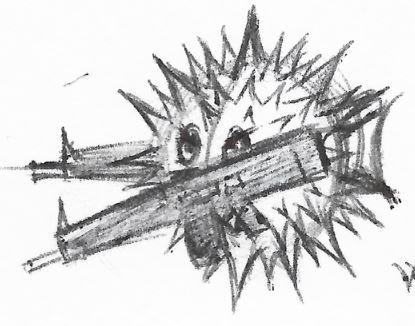
\includegraphics[height=10cm]{proactivesecurity/proactivesecurity.png}
	\caption[center]{.ni'o le nu mi'a pilno la'o gy.\ OpenBSD .gy cu zva'ati\@  .i doi fazgau do'u ko na troci}
\end{figure}
\section{le pamoi velski po le pixra}
.ni'o le jongau pixra cu sekibdu'a ki'u le nu filselga'e claxu lo pixra poi pixra la .pyfis.

.ni'o la .pyfis.\ claxu lo kalmebykre ki'u le nu mo'ifli le nu pixra lo kalmebykre

.ni'o la'o gy.\ AA-12 .gy u'enderfu xacyce'a
\chapter{la'o gy.\ WESTERNUNIONSOFTHECOUNTRYWESTERNS .gy}
\begin{figure}[ht]
	\centering
	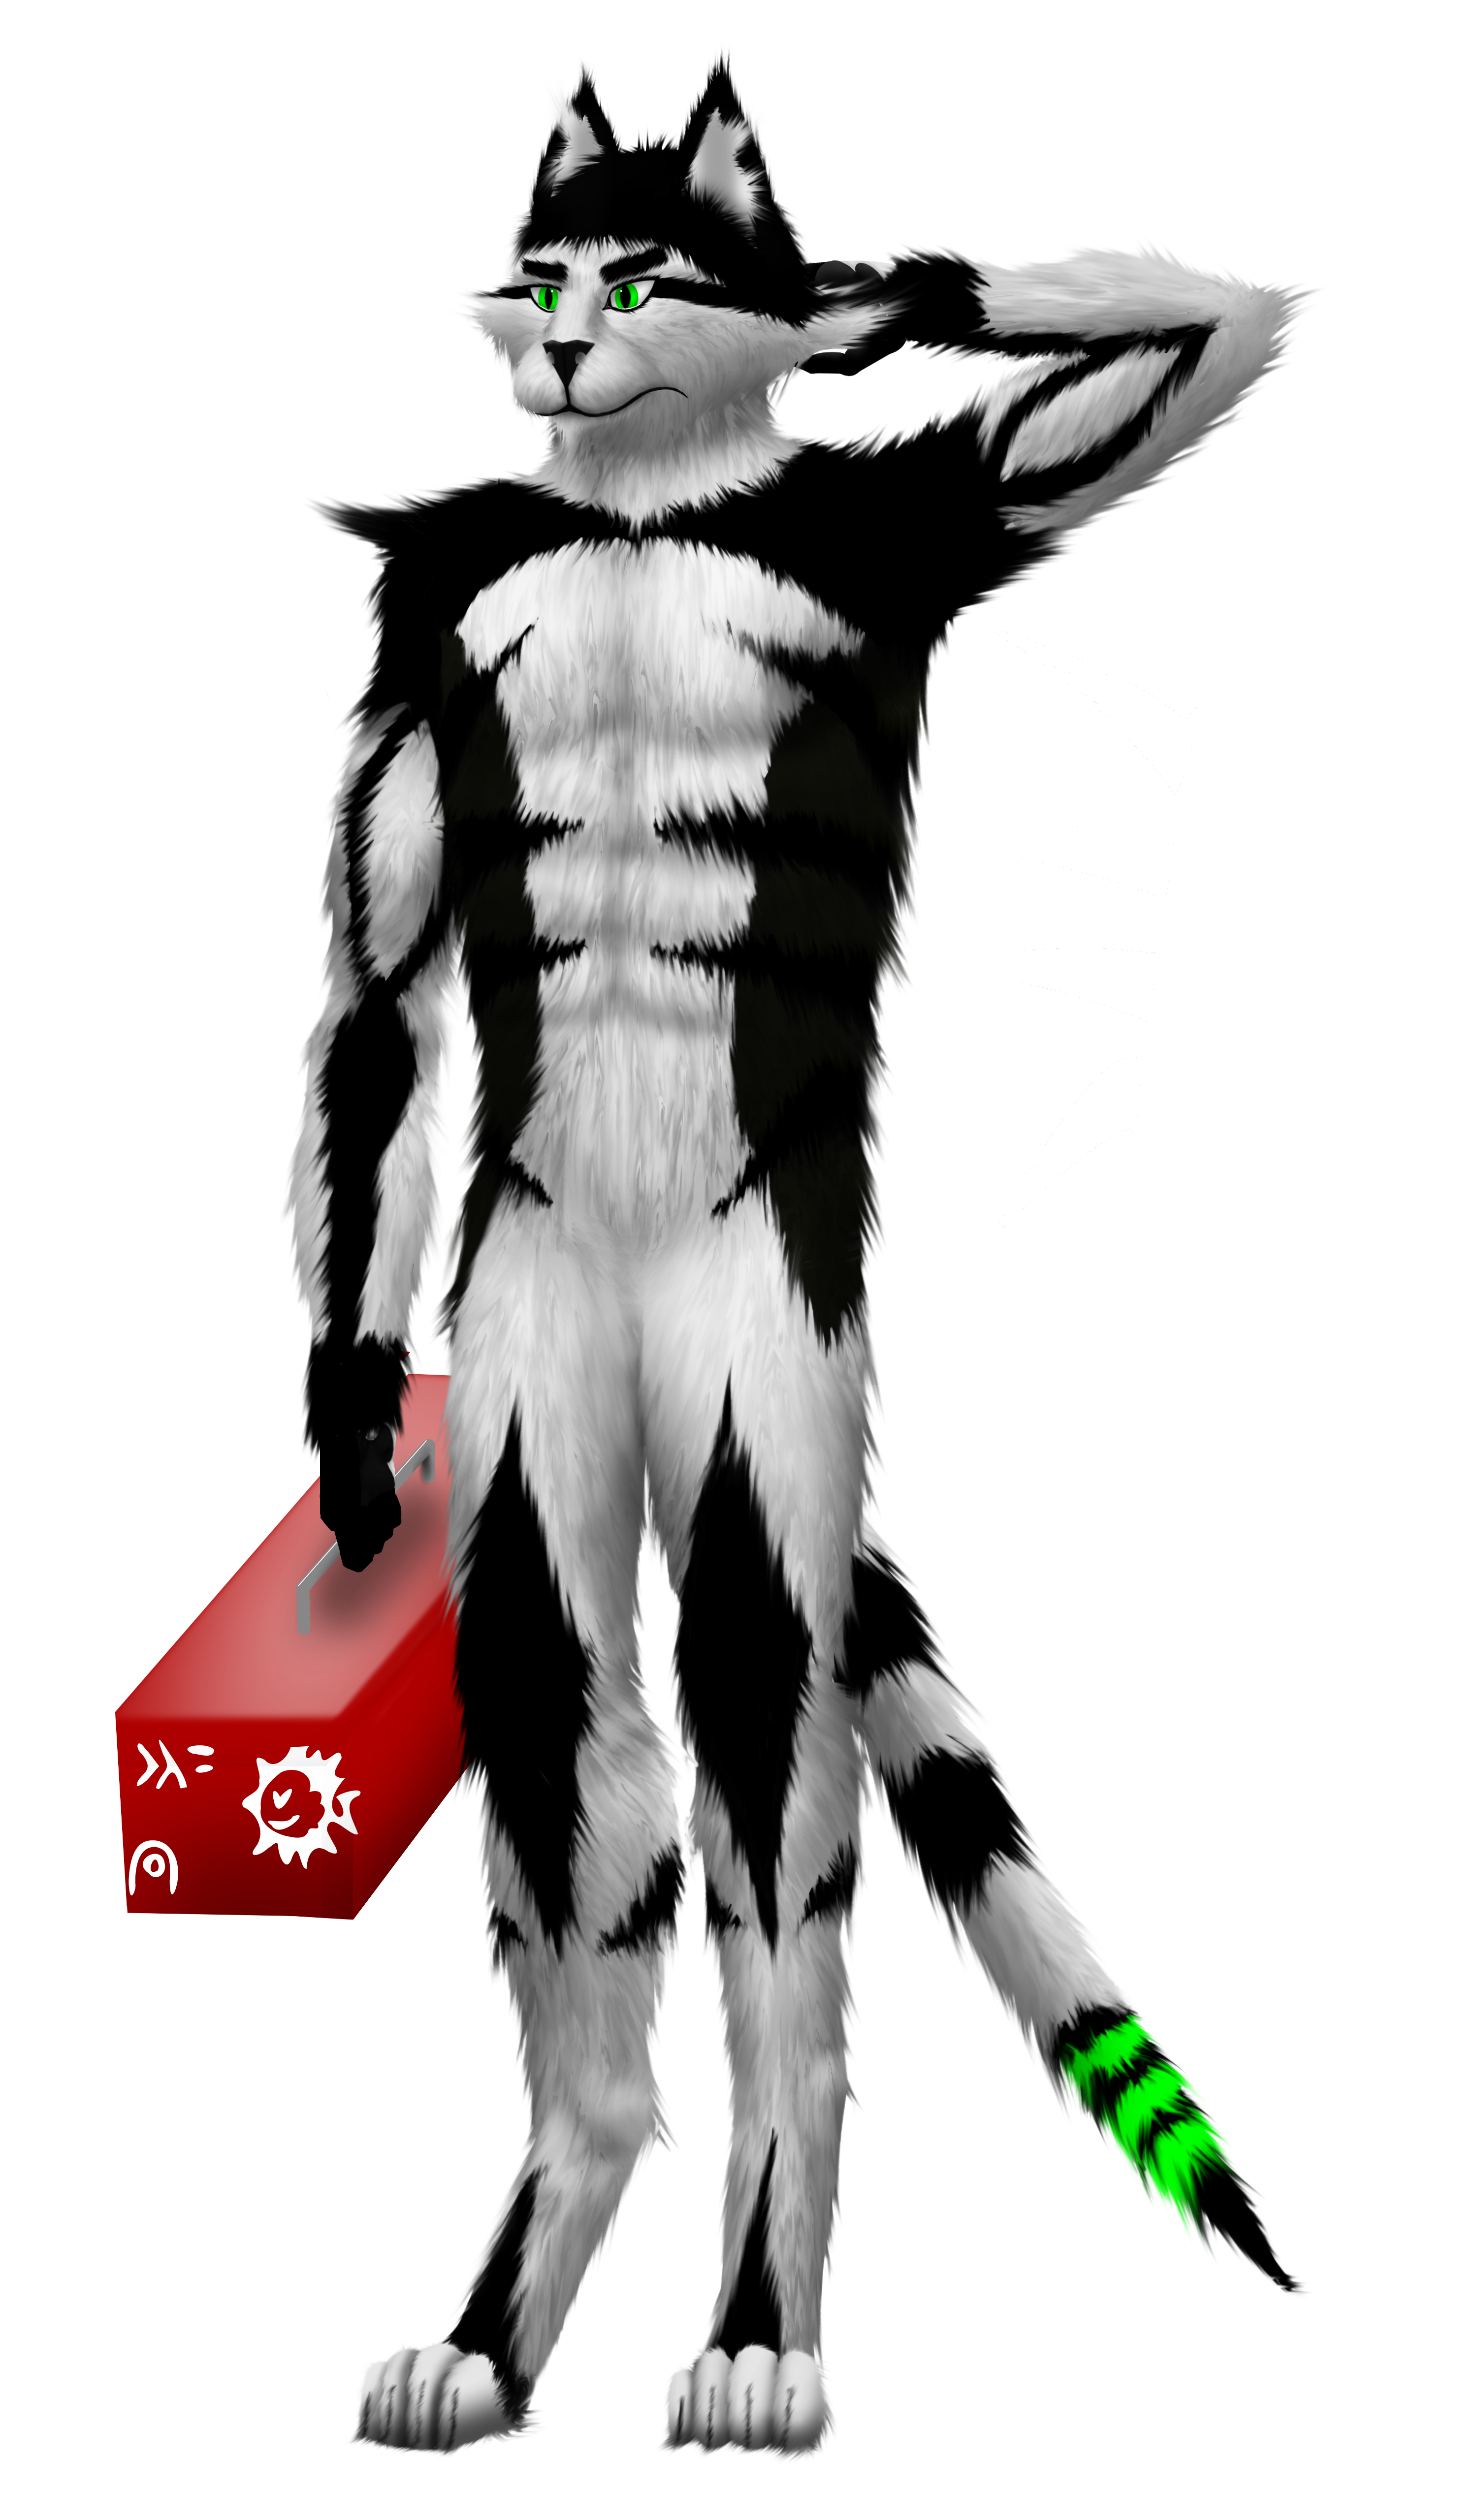
\includegraphics[height=\imageheight]{50x/toolbox/westernunionsofthecountrywesterns.png}
	\caption[center]{le pixra .e le na setcidu}
\end{figure}
\section{le pamoi velski po le pixra}
\subsection{lo snada ci fi'u vo zo'e}
.ni'o le nu la .varik. troci le nu pixra lo ci fi'u vo xarpre po la .varik. kei gi'e denpa fe le nu pixra cu semulcabna le nu la .varik. pixra lo ci fi'u vo xarpre po la .varik.
\subsection{le jacyba'a .e le pilno jaspu}
.ni'o ji'a ti poi pixra cu na mutce fanza se jacyba'a\@  .i ku'i ti poi pixra cu na sevasru la'o gy.\ public domain .gy\@  .i la .varik.\ ralte le krali po ti poi pixra\@  .i ku'i le nu li ni'e ni di'u jetnu lo'o selbi'o cu cumki\@  .i le nu le temci cu flecu pe'a cu cabna le nu li ni'e ni la .varik.\ nelci le nu la'o gy.\ public domain .gy vasru lo pixra lo'o zenba
\subsection{le pilno}
.ni'o pilno la'o gy.\ Krita .gy noi mutce to'e se nelci la .varik.

.ni'o le nu zbasu ti poi pixra cu cabna le nu la'o gy.\ Krita .gy goi ko'a ge'u nasru'e naspli masno\@  .i semupli le du'u le nu ko'a rinka le nu lo senta pe'a cu selvisnalka'e cu snidu li ji'i cino\@  .i le masna cu milxe serinka le nu la .varik.\ pilno la'o gy.\ GIMP .gy le nu zbasu lo balvi pixra\@  .i la .varik.\ ponse lo seplijaspu po la'o gy.\ CLIP STUDIO PAINT EX .gy gi'e zmanei la'o gy.\ CLIP STUDIO PAINT EX .gy la'o gy.\ Krita .gy lo so'e krinu\@  .i li ni'e ni la .varik.\ nelci la'o gy.\ WINE .gy po la'o gy.\ FreeBSD .gy lo'o ranji zenba

.ni'o le nu la'o gy.\ GIMP .gy ze'i pilno cu semulcabna le nu la'o gy.\ GIMP .gy claxu lo su'o jicmu poi sepilno la .varik.\@  .i le zmiku klina senta tadji cu semupli\@  .i krinu le nu la .varik.\ pilno la'o gy.\ Krita .gy le nu mulgau ti poi pixra
\subsubsection{lo zoi gy.\ open-source .gy sampla cu cumki xamgu}
.ni'o le zoi gy.\ open-source .gy sidbo cu senelci.\ gi'e cumki friti lo jetnu kalci pe'a\@\@  .i lu lo prenu poi to'e nelci ku'o cumki cikre lo samru'e li'u xlali krinu ki'u le nu su'o da poi pilno lo samru'e zo'u da na samru'e ciska\@\@  .i ji'a lo xlali samselpla cu zasti\@  .ije la .varik.\ na jinvi le du'u le samselpla po la'o gy.\ Krita .gy cizra xamgu

.ni'o le nambi cu secusku ki'u le nu la .varik.\ djica le nu la .varik.\ nelci la'o gy.\ Krita .gy .e la'o gy.\ GIMP .gy.\\@  .i ku'i la .varik.\ nelci la'o gy.\ Krita .gy .e la'o gy.\ GIMP .gy .inaja la'o gy.\ Krita .gy .e la'o gy.\ GIMP .gy sisti le nu kalci pe'a
\subsection{le sinxa}
.ni'o le nu sispe'i zo'e poi sesinxa le sinxa cu frili le tcidu
\subsection{le versiio bo jitro pilno}
.ni'o secumki le nu le citri po ti poi pixra ku sekibdu'a fi la'o gy.\ GitHub .gy\@  .i la .git.\ jitro ti poi ti pixra gi'e zbasu le mlitce barda citri bo datnyveiste
ku'i le nu le citri cu tolkli ku cumki ki'u le nu la .varik.\ djica le nu la .varik.\ frili cple'idju zo'e poi indika le du'u la .varik.\ pu zbasu ti poi pixra
\subsection{le nitpiki}
ni'o le xamgu nitpiki cu mutce senelci\@  .i ku'i la .varik.\ djica le nu le nitpiki cu tilcfu ki'u le nu la .varik.\ jinvi le du'u li ni'e ni lu le caltai po le birka ku ku namapti le ctino po le birka li'u goi ko'a sidju cu dubmau li ni'e ni lu le birka cu xlali li'u goi ko'e sidju\@  .i ku'i ko'a .e ko'e cumki sidju
\subsection{le pilno}
.ni'o pilno la'o gy.\ ed(1) .gy le nu ciska ti poi celski
\section{le xlali betfu bo sluji}
le caltai po le betfu sluji po la'o gy.\ VUNC .gy ku po la'o gy.\ WESTERNUNIONSOFTHECOUNTRYWESTERNS .gy xlali

.i le nabmi cu serinka le tadji po le nu pixra lo betfu sluji kei po la .varik.\ ku ku goi ko'a\@  .i ko'a pruce fo le nu pixra lo nonkansa pe'a sluji
\section{le sutra pirlarfi'i}
le lisri skina poi skicu le pruce po le nu zbasu la'o gy.\ WESTERNUNIONSOFTHECOUNTRYWESTERNS .gy cu kibzva la'o gy.\ \url{https://diode.zone/w/vR9yipHTfuaH3SKPiEXFLm} .gy .e la'o gy.\ \url{https://vimeo.com/635651456} .gy\@  .i ku'i ji'a lo gletu pe'a jifkri goi ko'a cu cumki catlu le skina ki'u le nu le skina kibzva la'o gy.\ \url{https://www.youtube.com/watch?v=0wyF7okop64} .gy
\subsection{le mabla skicu}
.ni'o le skina pagbu po le sutra pirlarfi'i cu milxe mabla le demri'a

.ni'o le xlali cu lakne sekrinu le nu la .varik.\ pilno le la'o gy.\ AVI .gy pruce poi claxu lo sumti ku'o po la'o gy.\ \textsc{ffmpeg} .gy goi ko'a le nu rejgau le lisri skina\@  .i ko'a pilno le mutce cirko bo rinka bo pruce po la'o gy.\ H.264 .gy
\section{le sirsunla tcila claxu}
.ni'o le sirsunla po la'o gy.\ VUNC .gy ge'u po ti poi pixra cu nacmatilcfu

.ni'o le nu zbasu la'o gy.\ WESTERNUNIONSOFTHECOUNTRYWESTERNS .gy cu cabna le nu la .varik.\ filba le nu jmina lo cmalu sirsunla bo tcila\@  .i le filba cu serinka le pixra poi sevasru noda .e le barda sirsunla tcila
\section{le tsautu}
\subsection{le pamoi tsautu}
.ni'o le pamoi versiio po la'o gy.\ WESTERNUNIONSOFTHECOUNTRYWESTERNS .gy cu milxo mabla pinsi bo tsautu
\begin{figure}[ht]
	\centering
	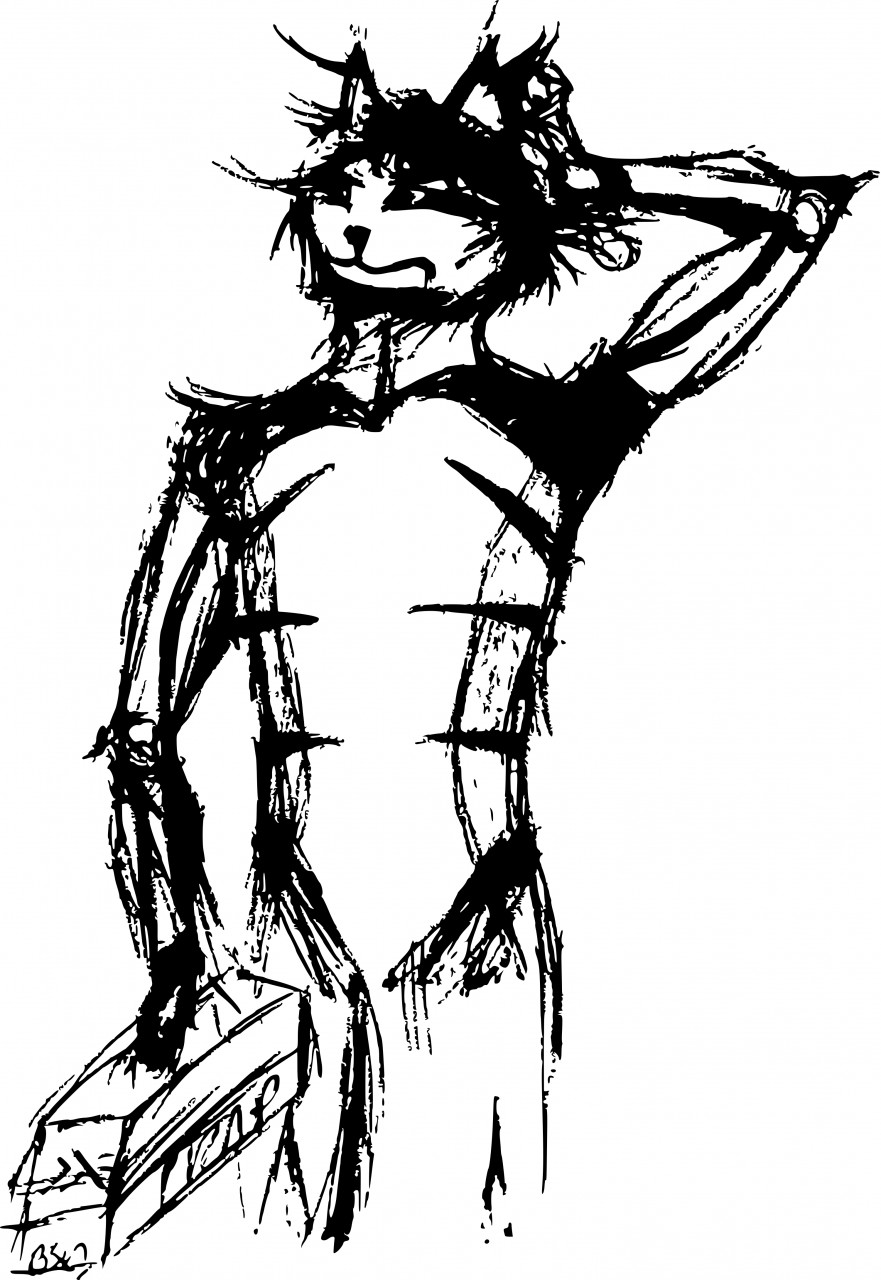
\includegraphics[height=\imageheight]{50x/toolbox/s1v1.jpg}
	\caption[center]{le pamoi versiio po la'o gy.\ WESTERNUNIONSOFTHECOUNTRYWESTERNS .gy}
\end{figure}
\subsection{le remoi tsautu}
.ni'o le pamoi tsautu po la'o gy.\ WESTERNUNIONSOFTHECOUNTRYWESTERNS .gy cu pamoi milxo xamgu pinsi bo tsautu\@  .i ku'i ti poi tsautu cu uaigri le vektori pixra poi kibzva la'o gy.\ \url{https://github.com/varikvalefor/drawingstuff/blob/master/50x/toolbox/toolboxsketch002.svg} .gy
\begin{figure}[ht]
	\centering
	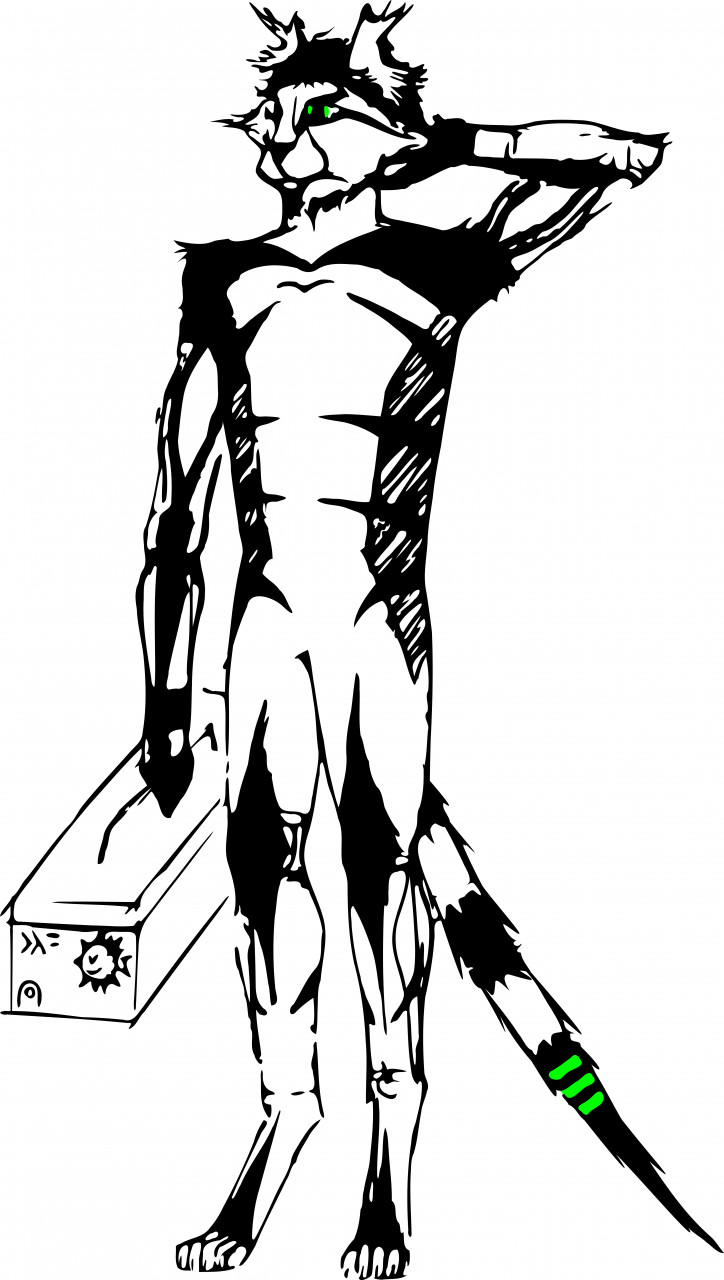
\includegraphics[height=\imageheight]{50x/toolbox/s1v2.jpg}
	\caption[center]{le pamoi tsautu po la'o gy.\ WESTERNUNIONSOFTHECOUNTRYWESTERNS .gy}
\end{figure}
\chapter{HOLLYWOODFREAKSONTHEHOLLYWOODSCENE}
\begin{figure}[ht]
	\centering
	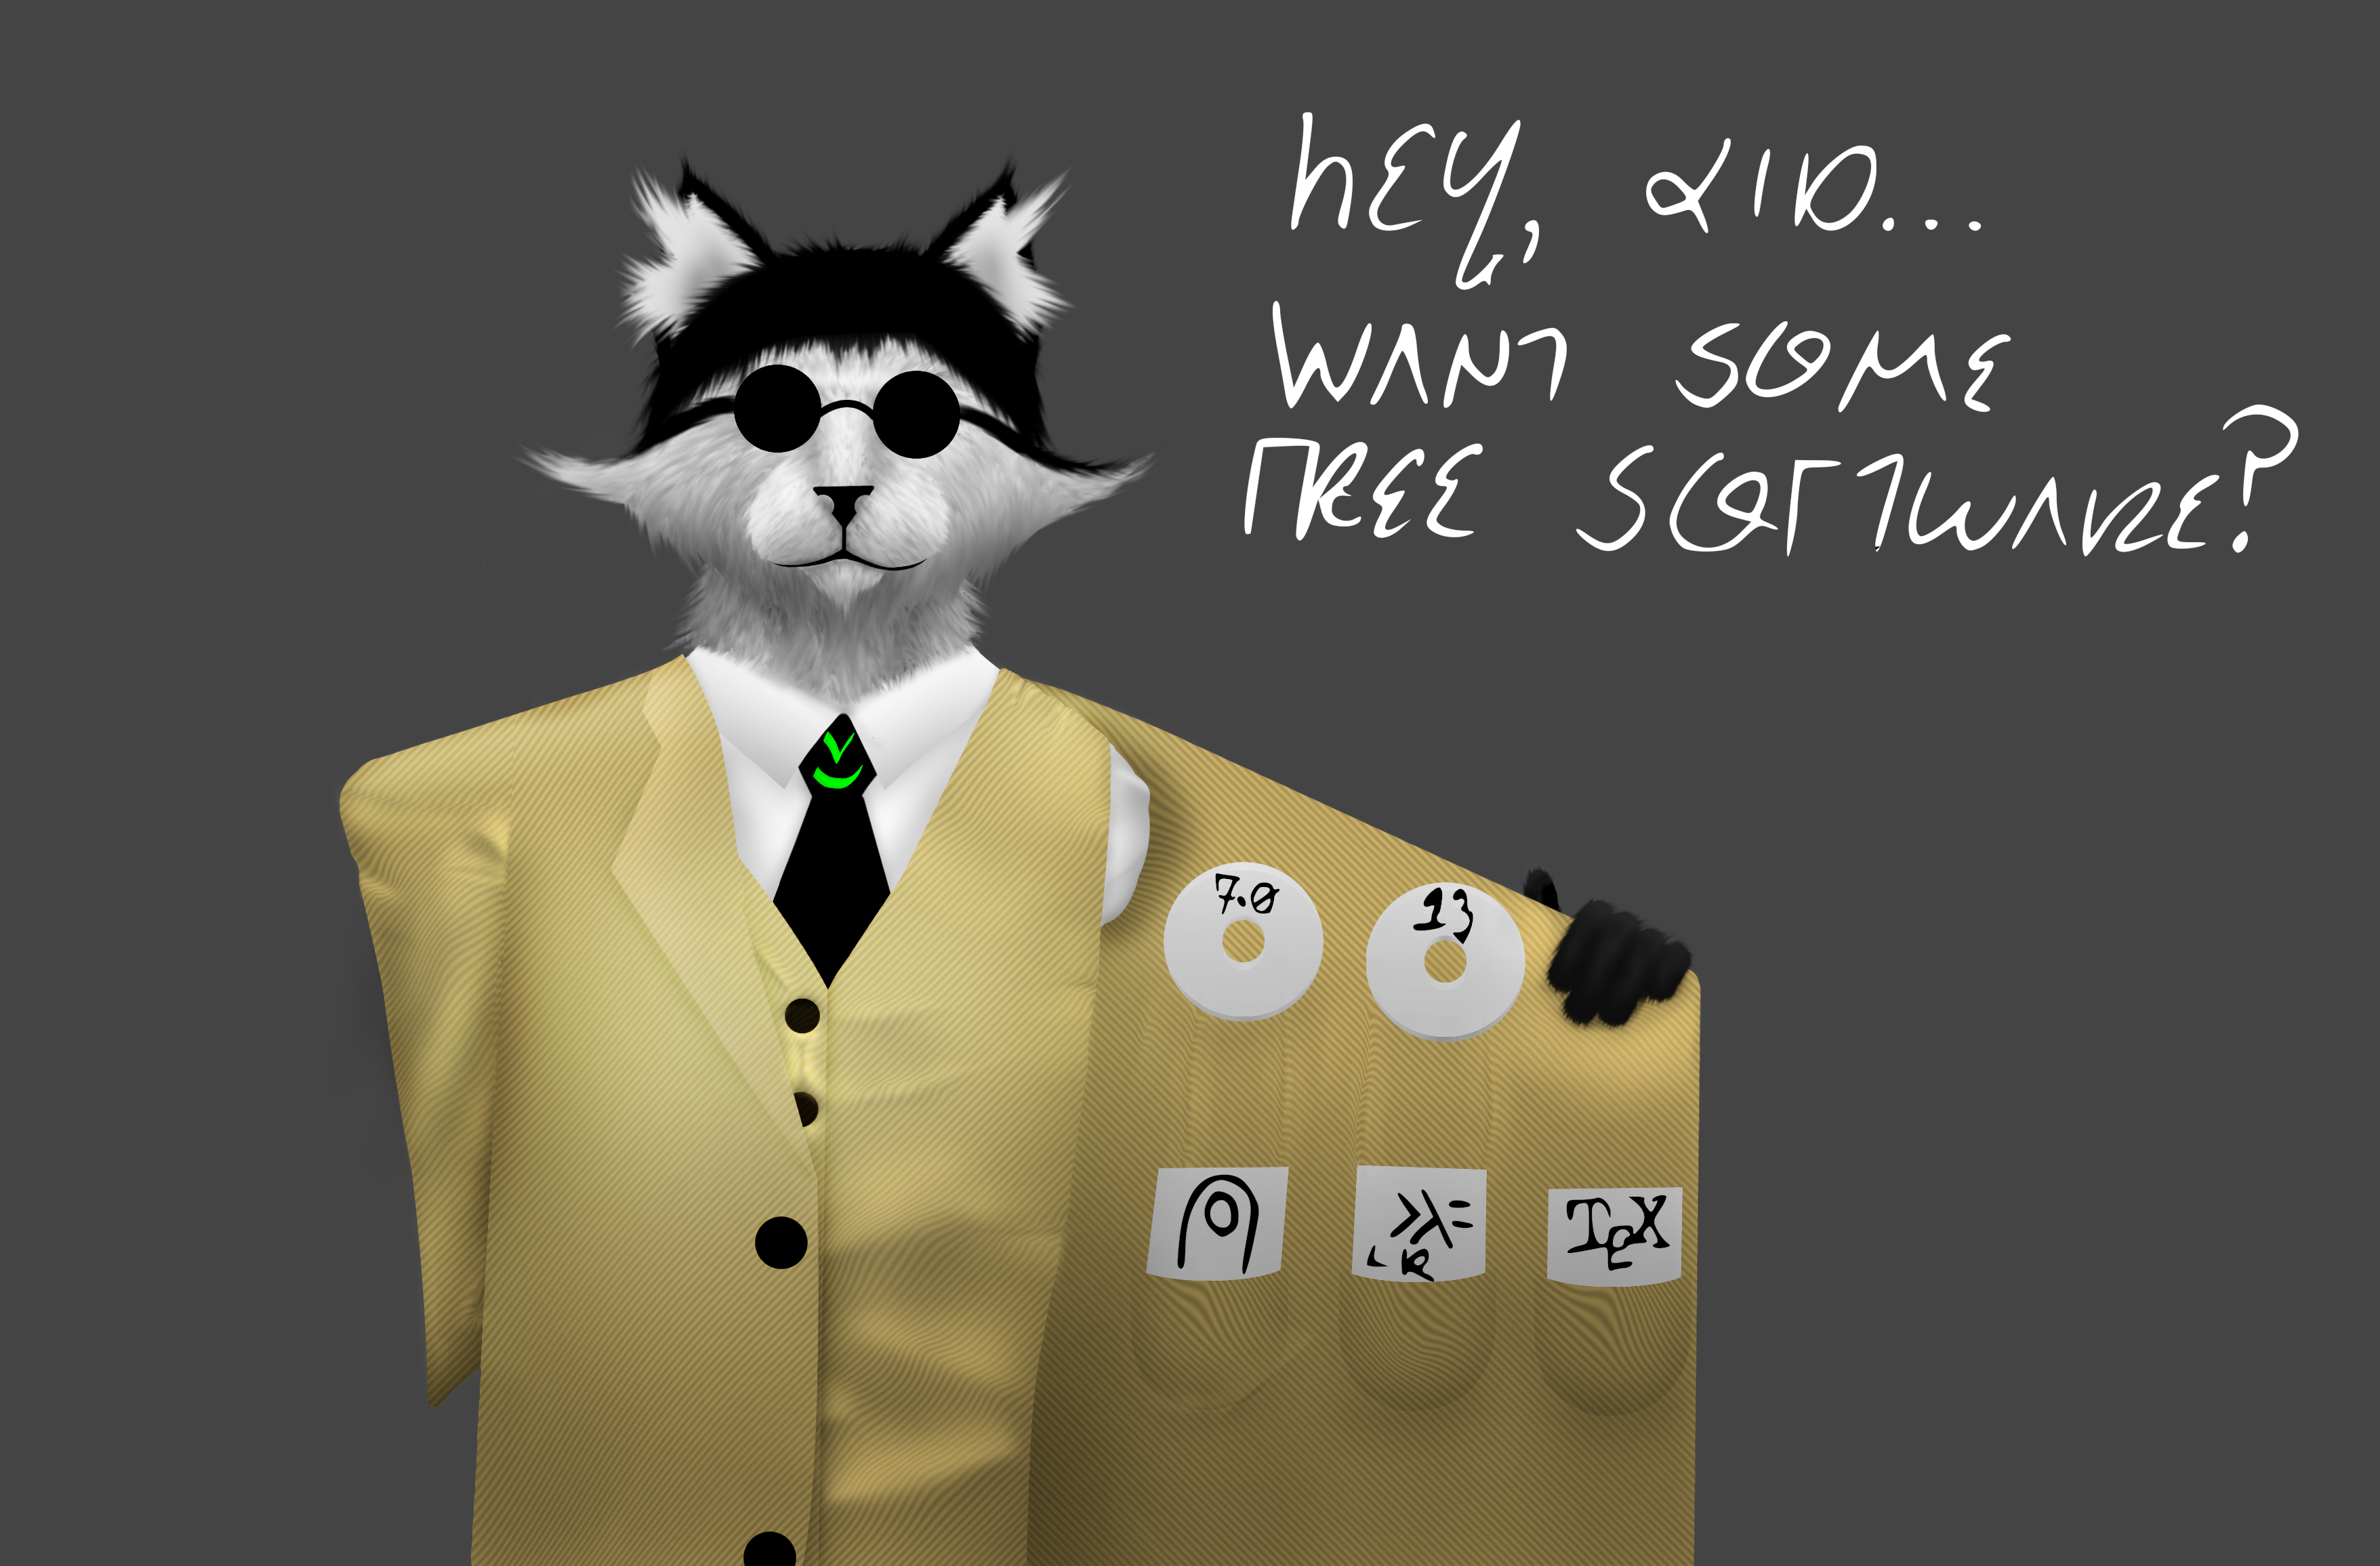
\includegraphics[height=\imageheight]{hollywoodfreaksonthehollywoodscene/hollywoodfreaksonthehollywoodscene.png}
	\caption[center]{``HOLLYWOODFREAKSONTHEHOLLYWOODSCENE''.}
\end{figure}
\section{The Original Description of the Drawing}
\subsection{A Cheesy-Ass Short Story}
Let there exist a man $J$.

$K$ denotes the depicted man.

In the middle of an arbitrary night, as $J$ walks down an arbitrary street and nears a power substation, $K$ appears from behind a bush and slowly approaches $J$.

Whilst $J$ appears rather surprised and unnerved, $K$ opens $K$'s coat and speaks the following words: ``Hey, kid\ldots want some free software?''

Determining whether or not $J$ ``takes up'' $K$'s offer is left as an exercise for the reader.
\subsection{Blah}
Another dumb joke is revealed!  In this case, the joke takes the form of a drawing which is called ``HOLLYWOODFREAKSONTHEHOLLYWOODSCENE''.

In addition to being a dumb joke, this drawing is VARIK's first \textit{real} attempt to draw fabric.
\subsection{The Contents of the Coat}
\subsubsection{Discs}
The ``7.0'' disc is an OpenBSD installation disc, and the ``13'' disc is a FreeBSD installation disc.  As of the publishing of this drawing, 7.0 and 13.0 are the most recent versions of OpenBSD and FreeBSD, respectively.
\subsubsection{Coat Pockets}
The reader can assume that the contents of the pockets of the coat are specifications and compilers of the programming languages whose ``logos'' are mentioned.  ``[L]ogos'' is written in inverted commas because one such ``logo'' is not an established logo but is a recognisable feature of the programming language which this ``logo'' represents.
\subsubsection{On the Amount of Stuff}
Whilst conceptualising this drawing, VARIK intends to mention a relatively great number of softwares.  However, there exists an idea such that this idea does not immediately come to fruition.  A ``deluxe'' version of this drawing may eventually be created.
\subsection{Criticism}
As ever, criticism regarding this drawing is appreciated.
\subsection{Tools Used}
This drawing is drawn using GIMP\@.

This description is written using ed(1).
\section{Two-Dimensional Appearance of Clothing}
Several men claim that in ``HOLLYWOODFREAKSONTHEHOLLYWOODSCENE'', VUNC's clothing lacks depth and appears to be paper or something.

VARIK agrees with this assessment.

Luckily, the idea of wearing a paper suit which lacks a back is damn funny.
\section{Shading of Discs}
VARIK finds that the discs resemble paper cut-outs, as opposed to optical discs.  This problem may result from the discs' complete opacity.
\chapter{BROKEDOWNOUTINADITCHOFOLDRUBBISH}
\begin{figure}[ht]
	\centering
	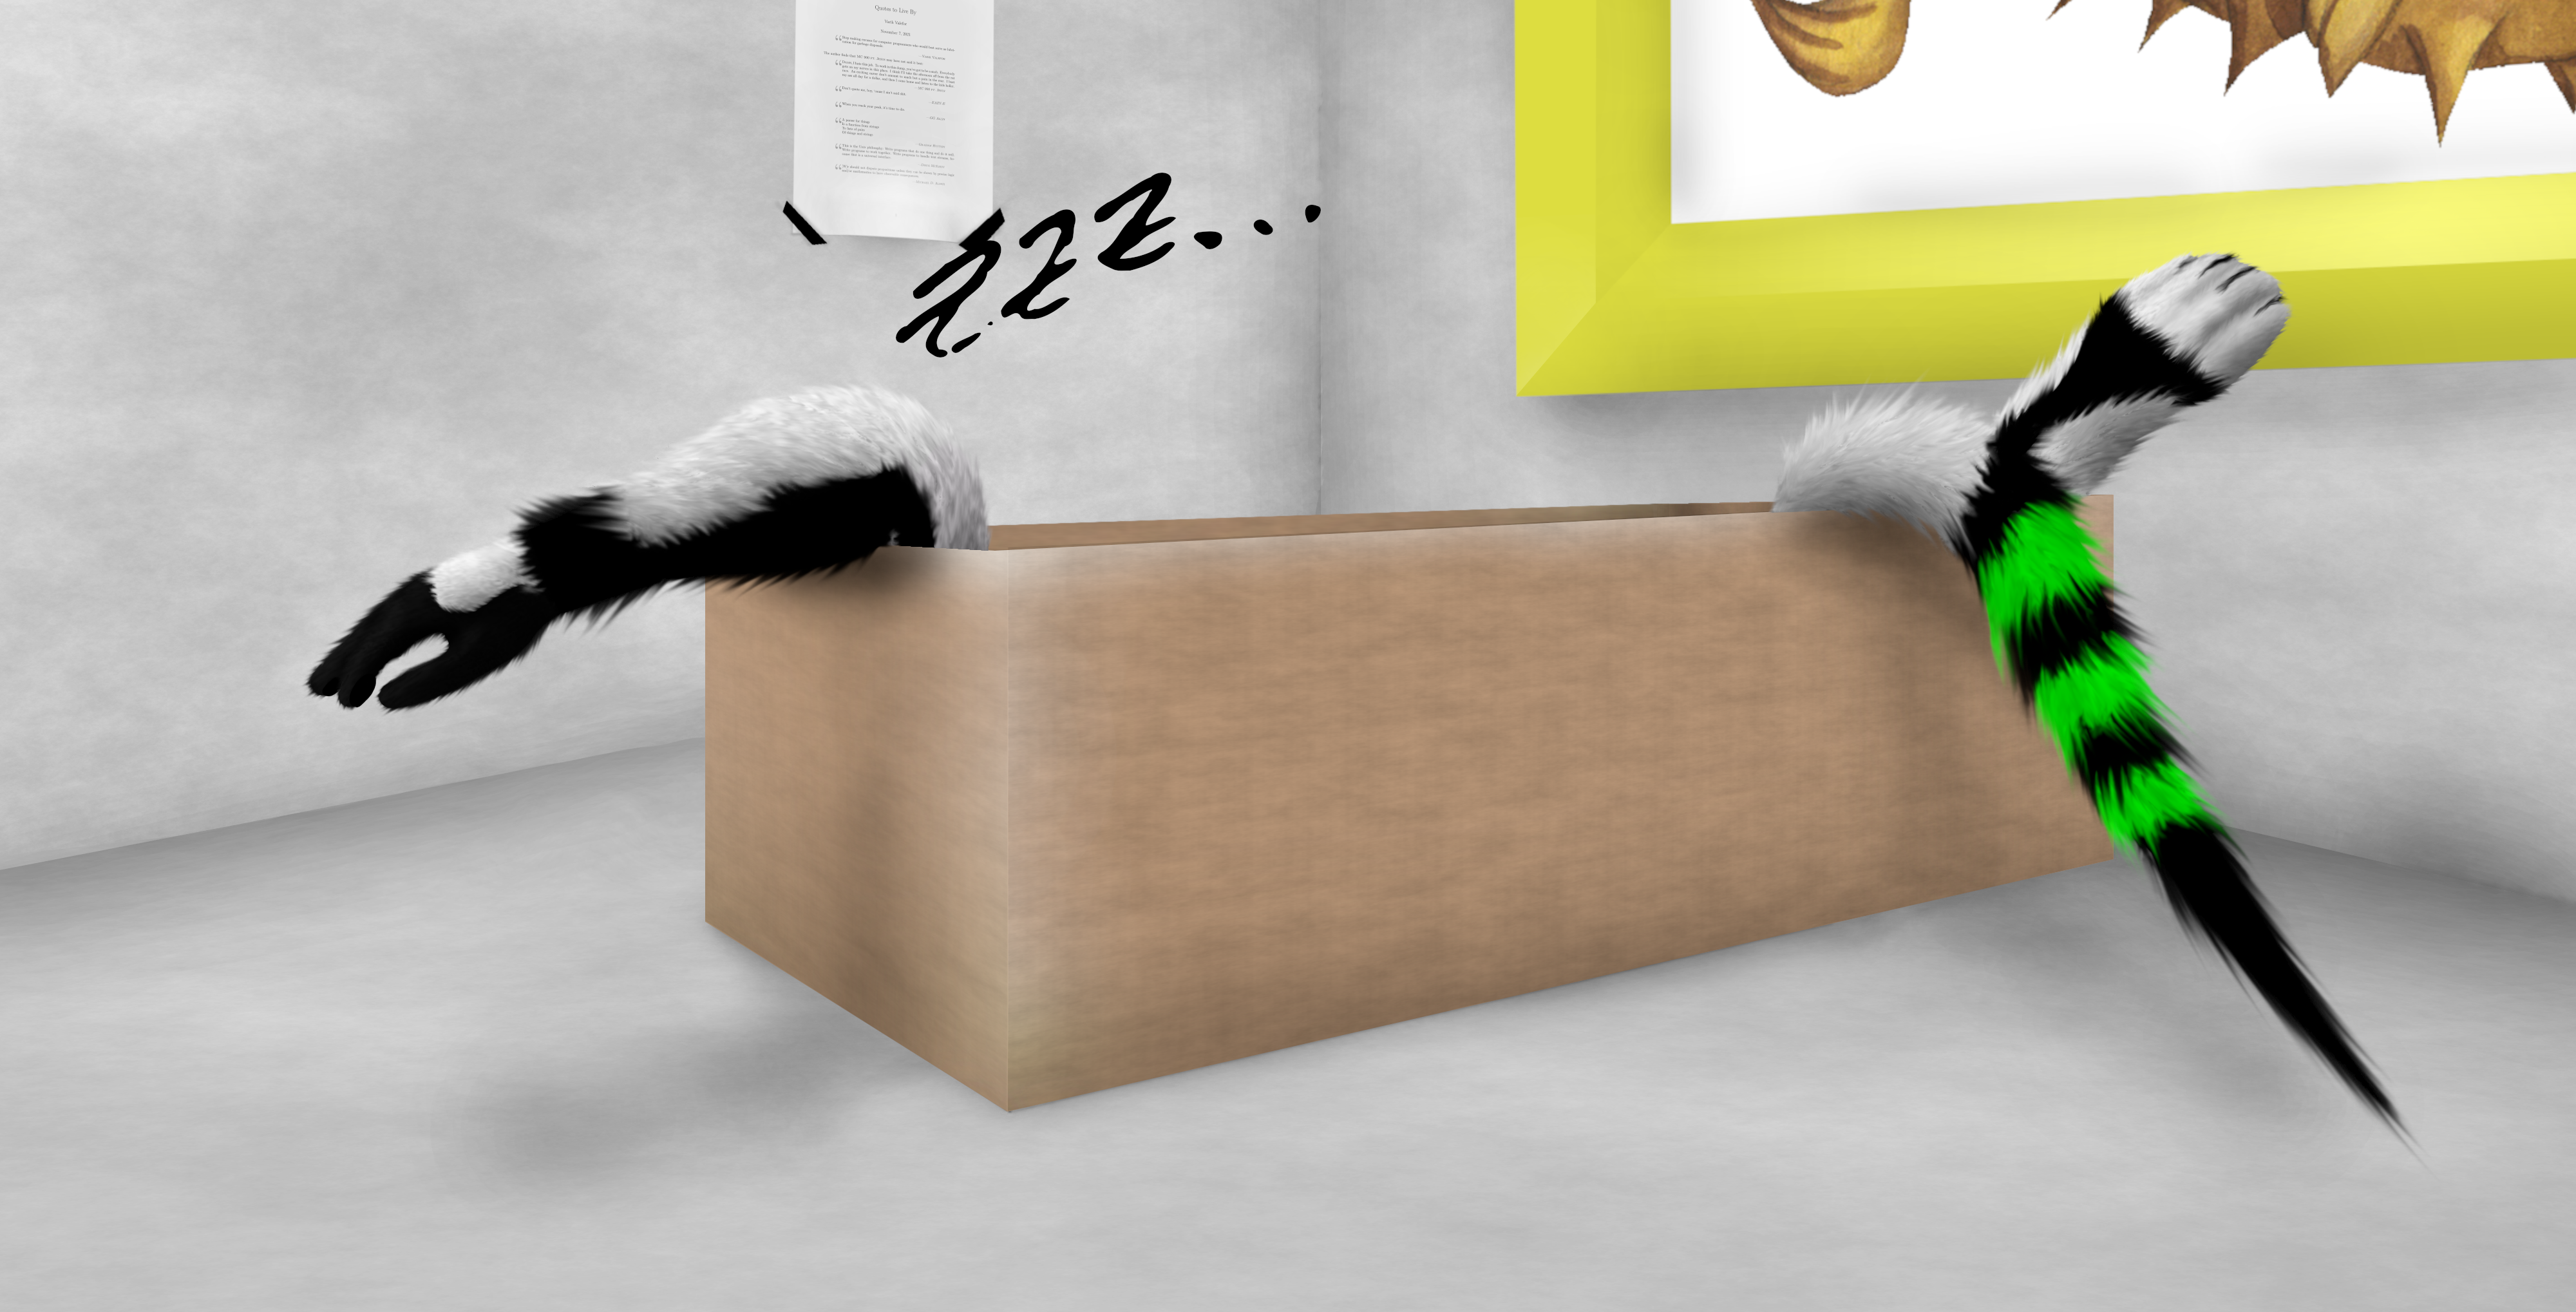
\includegraphics[width=\textwidth]{brokedownoutinaditchofoldrubbish/brokedownoutinaditchofoldrubbish.png}
	\caption[center]{This figure is the drawing.  Is a photograph of a ham sandwich or something expected?  Have some sense, foo'.}
\end{figure}
\section{The Original Description of the Drawing}
A new drawing is revealed!

\subsection{``Proper'' Background\ldots and Jokes}
This drawing, which is called ``BROKEDOWNOUTINADITCHOFOLDRUBBISH'', is VARIK's first published drawing which features a ``proper'' background, as opposed to a solid colour or some abstract thing.  Additionally, ``BROKEDOWNOUTINADITCHOFOLDRUBBISH'' includes a few jokes.

\subsection{On the Box}
The reader can assume that the cardboard box in which the character lies is reinforced such that this box is not deformed under minor weight.  The reader can also assume that the flaps of this box are folded inward or removed.

\subsection{Origins as an Inside Joke}
This drawing actually begins as an inside joke, as the box is originally adorned with some text which functions as an inside joke.  However, VARIK eventually concludes that this inside joke is not terribly amusing and removes the part of the drawing which qualifies as an inside joke.

\subsection{On ``ZZZ\ldots''}
The presence of ``ZZZ\ldots'' indicates that the character is snoring, which indicates that the character is sleeping.  But why in the hell is ``ZZZ\ldots'' the accepted transcription of snoring?

\subsection{Criticism}
As ever, criticism is appreciated.

\subsection{Weapons of Choice}
This drawing is created using GIMP\@.  The actual drawing work is done with a trackpad.

This description is written using ed(1).

Both GIMP and ed(1) are run on OpenBSD\@.
\chapter{DANCINGONTHEROOFSHOOTINGHOLESINTHEMOON}
\begin{figure}[ht]
	\centering
	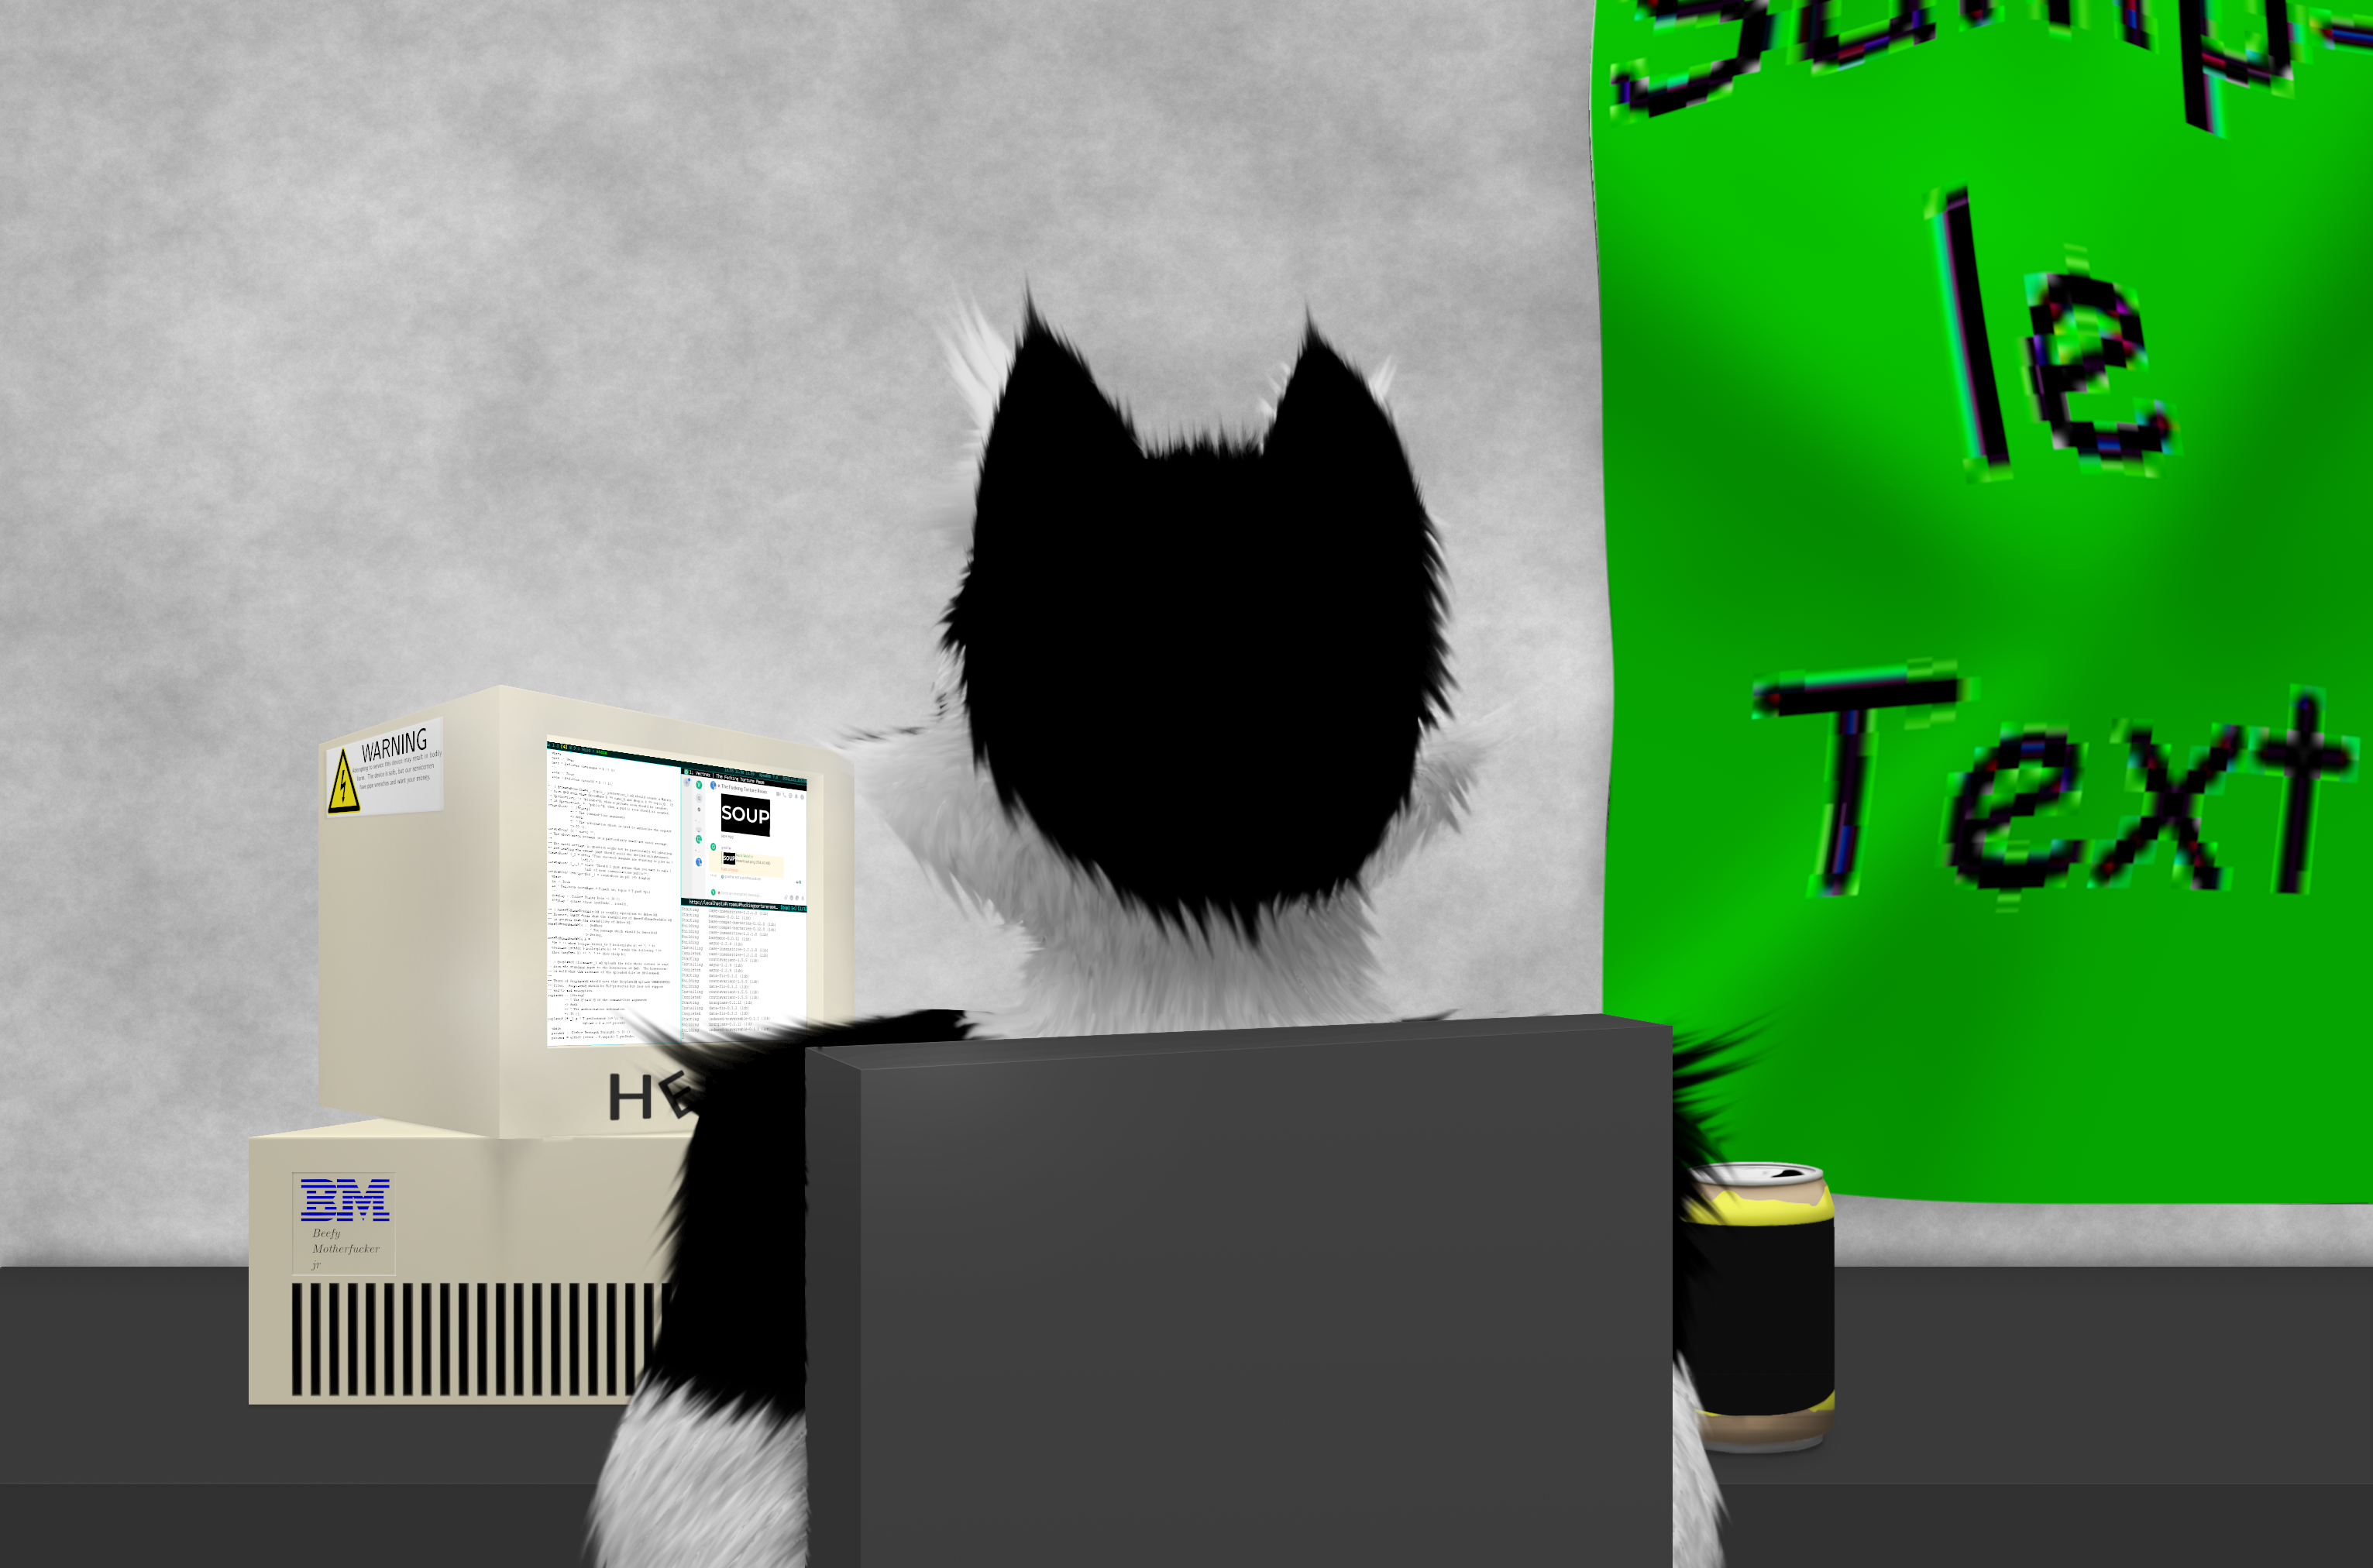
\includegraphics[width=\textwidth]{dancingontheroofshootingholesinthemoon/dancingontheroofshootingholesinthemoon.png}
\caption[center]{The full version of ``DANCINGONTHEROOFSHOOTINGHOLESONTHEMOON''.  To see every detail, use a magnifying glass\ldots or a microscope.}
\end{figure}
\section{The Original Description of the Drawing}
Yet another drawing is created!
In this case, the drawing depicts an everyday situation\ldots but is hopefully not too boring.
\subsection{Definitions}
Let ``VUNC'' denote VARIK's character.
\subsection{Executive Summary}
In this drawing, VUNC sits at a terminal and works on some tedious software-related stuff\ldots whilst reading terrible chatroom messages.
\subsection{Jokes and Whatnot}
Like VARIK's other drawings, this drawing features a decent number of jokes and references.  Explaining these jokes is left as an exercise for the reader.
However, in addition to some jokes, this drawing contains a small social commentary.  Describing this social commentary is \textit{also} left as an exercise for the reader.
\subsection{On ``SOUP''}
The stupid-looking ``SOUP'' image on the display is present because VARIK is uncertain of whether or not the original image can be included freely in the drawing.  To prevent a lawsuit or the threat of a lawsuit, a ``description'' of the possibly copyrighted image replaces the possibly copyrighted image.

``[D]escription'' is written in inverted commas because this ``description'' is not terribly descriptive.  A relatively descriptive description of the original image is ``a heavily-compressed photograph of a bowl of alphabet soup''.
\subsection{Warning Label}
The full text of the warning label is as follows:
\begin{quote}
	WARNING

	Attempting to service this device may result in bodily harm.  The device is safe, but our servicemen have pipe wrenches and want your money.
\end{quote}
\subsection{Keyboard}
In the depicted scene, VUNC uses a keyboard.  However, this keyboard is not visible, and VUNC's use of this keyboard could probably be relatively well indicated.
\subsection{Criticism}
As ever, criticism is welcomed.
\subsection{Licence}
This drawing is released in accordance with the CC BY-NC 4.0 licence.  The full text of this licence is available at \url{https://creativecommons.org/licenses/by-nc/4.0/legalcode}.
\subsection{Tools Used}
This drawing is created using GIMP\@.  GIMP is terrible but seems to be the best open-source drawing software.

This description is written using ed(1).

Both GIMP and ed(1) are run on OpenBSD\@.
\section{Chair}
The chair which VUNC uses lacks detail; the material of the chair is ambiguous.  The design of the chair is mostly style-based, as VARIK strongly likes brutalist architecture; however, regardless of the style, the chair just looks a bit cheesy.
\chapter{ITHINKWEREGOINGCRAZY}
\begin{figure}[ht]
	\centering
	\includegraphics[height=10cm]{ithinkweregoingcrazy/ithinkweregoingcrazy.png}
	\caption[center]{``ITHINKWEREGOINGCRAZY''.}
\end{figure}
\section{The Original Description of the Drawing}
BLOCKED BY SHODAN LEVEL SECURITY\@.
\subsection{``What the Hell am I Looking At?''}
This drawing depicts VARIK's character's being connected to some cables and having a neutral facial expression a la \textit{System Shock}'s SHODAN\@.
\subsection{Timing}
December apparently has at least one (1) drawing, as well.
\subsection{History}
\subsubsection{The Sketch}
Approximately fifteen (15) quintillion years ago, VARIK reveals a sketch which features VUNC hooked up to some cables a la \textit{System Shock}'s SHODAN\@.
\subsubsection{The First Attempted Conversion}
In early 2021, VARIK begins to convert this sketch into a ``proper'' drawing.  However, before VARIK backs up the drawing, VARIK accidentally deletes the master boot record of the hard disk drive of VARIK's terminal.  As a result of this mistake, the original version of the ``proper'' drawing is probably lost forever.
\subsubsection{The Second Attempted Conversion}
On 20210411, VARIK begins the process of converting the sketch into a ``proper'' drawing by adding the un-furred outlines of VUNC to a Scalable Vector Graphics file.  This process is finished with minimal ``hiccups''.
\subsubsection{Attempting to Add Detail}
Circa 20210602, VARIK converts the aforementioned SVG file into an XCF file and begins to add some detail.  For some reason, such detail is added before the cables are added.

Although few ``real'' problems are encountered, VARIK does not particularly care for the end result of the addition of such detail and pauses the creation of the drawing.
\subsubsection{Successfully Adding Detail}
On 20211127, VARIK resumes the creation of the drawing.  VARIK encounters few ``real'' problems but again concludes that GIMP can be a real turd\ldots figuratively.
\subsubsection{Finishing the Drawing}
On 20211201, VARIK declares that this drawing is finished.
\subsection{On this Drawing's Nature as an Amalgamation}
\textit{System Shock}'s SHODAN SHODAN serves as the direct inspiration of the creation of the SHODAN-``inspired'' parts of this drawing.  However, VARIK uses no particular SHODAN design as a reference whilst creating this drawing; VARIK bases this drawing upon a mental combination of SHODAN's \textit{System Shock} and \textit{System Shock 2} designs.
\subsection{Criticism}
As ever, criticism is welcomed.
\subsection{Licence}
This drawing is released in accordance with the CC BY-NC 4.0 licence.  The full text of this licence is available at \url{https://creativecommons.org/licenses/by-nc/4.0/legalcode}.
\subsection{Tools Used}
This drawing is created using GIMP\@.  GIMP is terrible but at least beats Krita.

This description is written using ed(1).

Both GIMP and ed(1) are run on OpenBSD\@.
\section{Eyestrain}
There exists a subset of all men $K$ such that for all $a \in K$, $a$ claims that $a$'s viewing of ``ITHINKWEREGOINGCRAZY'' results in the eyestrain of $a$.  VARIK suspects that men of $K$ are exaggerating things or have some weird eye problem; VARIK is incapable of finding any particular source of the eyestrain.
\section{Reception}
In short, ``ITHINKWEREGOINGCRAZY'' is relatively unpopular\ldots possibly because the ``source material'' of ``ITHINKWEREGOINGCRAZY'' is a bit obscure.
\subsection{Description of Reception}
The mean warmth of the reception of ``ITHINKWEREGOINGCRAZY'' is less than the mean of the warmths of the receptions of all drawings which VARIK creates.
\subsection{Possible Cause of Lukewarm Reception}
VARIK suspects that the relatively lukewarm reception of ``ITHINKWEREGOINGCRAZY'' may be a result of the relatively obscure nature of ``ITHINKWEREGOINGCRAZY''.
\begin{thm}
``ITHINKWEREGOINGCRAZY'' likely has a lukewarm reception.
\end{thm}
\begin{proof}
${}$

For all things $a$, for all drawings $b$, for all men $m$, $b$ is a parody of $a$ only if ($m$ fully understands $b$ only if $m$ is familiar with $a$).

For all drawings $b$, few men fully understand $b$ only if $b$ likely has a lukewarm reception.\footnote{The reader should probably take this statement with the proverbial grain of salt.}

Few men are familiar with \textit{System Shock}.\footnote{``Few'' may be an understatement.}

``ITHINKWEREGOINGCRAZY'' is a parody of \textit{System Shock}.

Therefore, ``ITHINKWEREGOINGCRAZY'' likely has a lukewarm reception.
\end{proof}
\chapter{la'o gy.\ JUDASTRAINWRECK .gy}
\begin{figure}[ht]
	\centering
	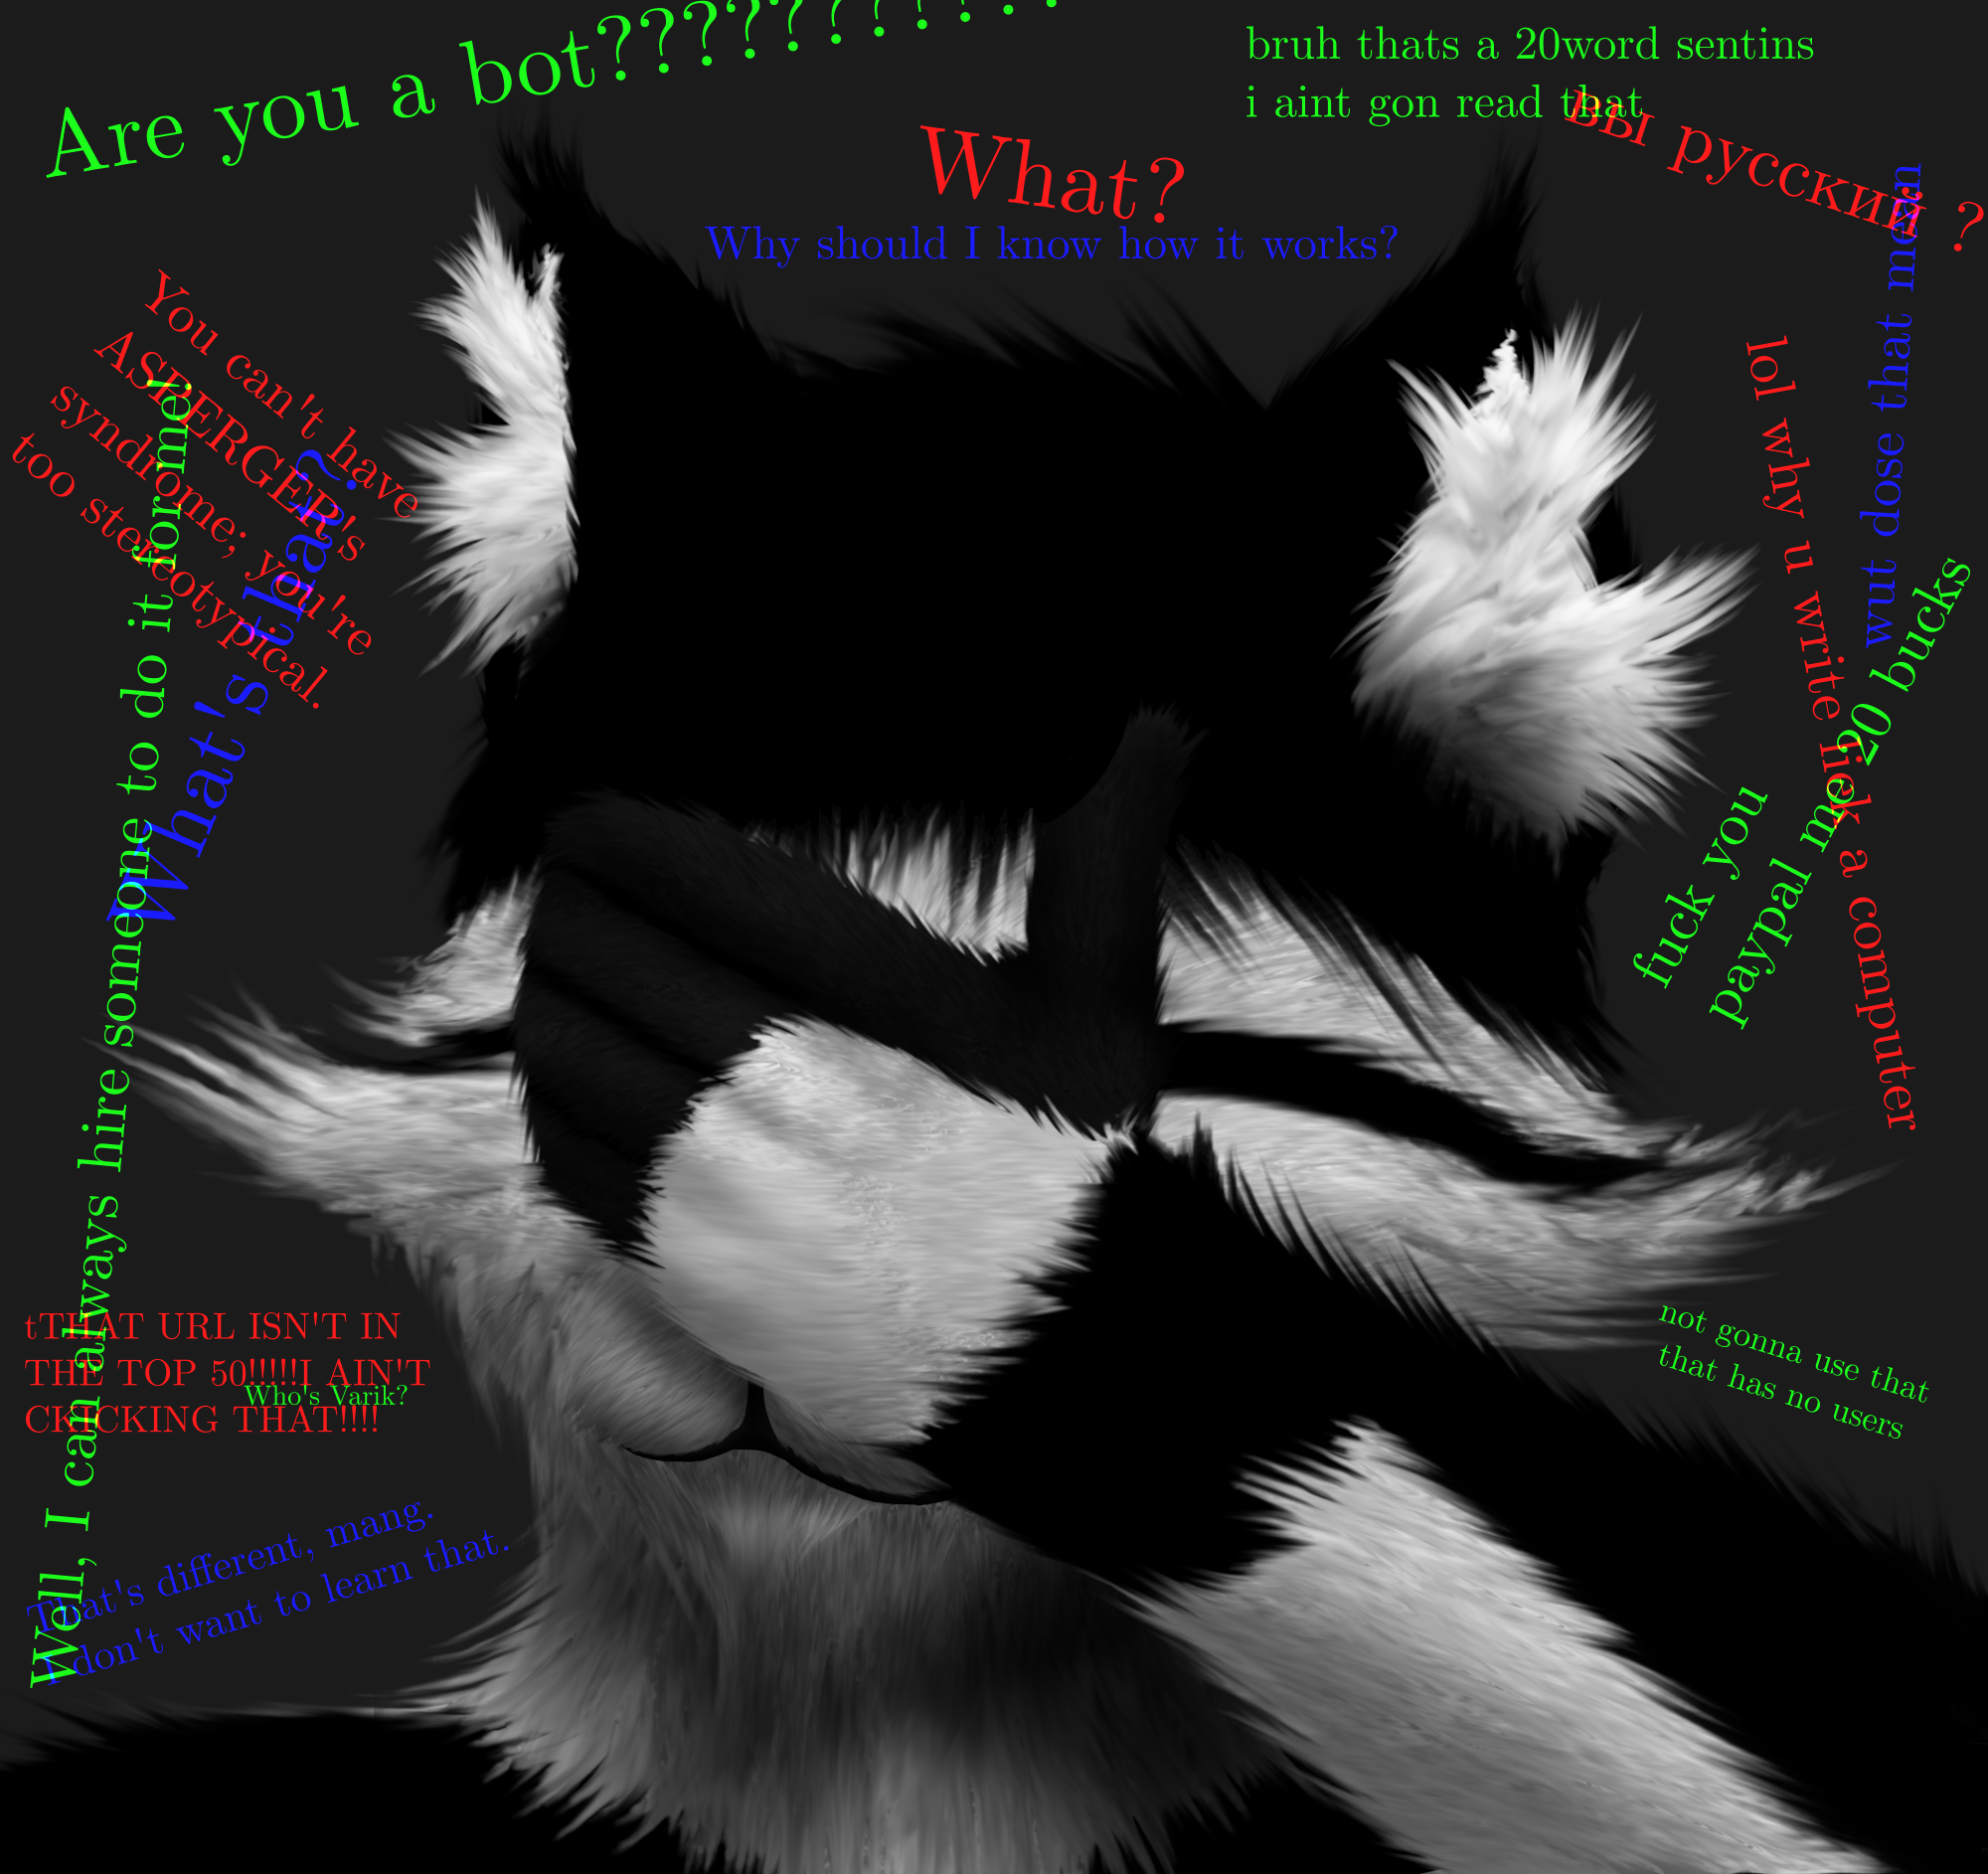
\includegraphics[height=10cm]{judastrainwreck/judastrainwreck.png}
	\caption[center]{la'o gy.\ JUDASTRAINWRECK .gy}
\end{figure}
\section{le pamoi velski po ti poi pixra}
la .varik.\ jinvi le du'u le firxa'e cu melbi
\subsection{le torveki}
.ni'o su'o da poi papri bo pixra tsautu zo'u da binxo le vektori pixra poi binxo ti poi pixra

.i le tcidu tanxe pe'a vasru lo toltce bo galfi notci poi pu seterbe'i la .varik.

.i ti poi pixra cu sexrapra gi'e seplijaspu la'o gy.\ CC BY-NC 4.0 .gy

.i doi la'o gy.\ lamer .gy ko pilno la'o gy.\ OpenBSD .gy
\subsection{le pruce poi gasnu le nu le tsautu ku binxo le mulno pixra}
.ni'o la .varik.\ majgau le pamoi tsautu ki'u le nu la .varik.\ djica le nu la .varik.\ terxra lo nasteci

.i la .varik.\ gasnu le nu le pamoi tsautu cu binxo le vektori pixra ki'u le nu la .varik.\ djica le nu la .varik.\ terxra zo'e poi trina

.i le nu la .varik.\ terxra le cabna pixra cu milxe sekrinu le nu la .varik.\ djica le nu la .varik.\ ckasu lo prenu poi cusku lo bebna preti.\ gi'a bebna pensi
\subsection{le tcidu tanxe pe'a}
.ni'o le tcidu tanxe pe'a vasru lo toltce bo galfi notci poi pu seterbe'i la .varik.

.i le nu la .varik.\ fuktra le cmoni po la'o gy. SIDESHOW BOB .gy cu sebalvi le nu la .varik.\ jdice le du'u le nu la .varik.\ ckasu le prenu gi'e curmi le nu le prenu ku cmecau cu filri'a le nu cmila
\subsection{le seplijaspu}
.ni'o ti poi pixra cu sexrapra gi'e seplijaspu la'o gy.\ CC BY-NC 4.0 .gy\@ .i le mulno tcidu po ti poi seplijaspu cu xabju pe'a la'o gy.\ https://creativecommons.org/licenses/by-nc/4.0/legalcode .gy
\subsection{le pilno}
.ni'o pilno la'o gy.\ GIMP .gy le nu majgau ti poi pixra\@ .i  la'o gy.\ GIMP .gy xlatce\@ .i ku'i zmanei la'o gy.\ GIMP .gy la'o gy. Krita .gy

.i ciska dei fo la'o gy.\ ed(1) .gy

.i la'o gy.\ GIMP .gy .e la'o gy.\ ed(1) .gy bajra pe'a la'o gy.\ OpenBSD .gy
\end{document}
